\section{Regular expression with complement and intersection}

Regular expressions may also contain the operators of complement, intersection and set difference, which are very useful to make the regular expression more concise. 
The family REG is closed under complement, intersection, and set difference. 

\subsection*{Complement}
The complement of a language $L$ is defined as: 
\[\lnot L = \Sigma^{*} \backslash L\]
Assume the recognizer $M$ of $L$ is deterministic, with initial state $q_0$, state set $Q$, set of finals states $F$ and transition function $\delta$. 
To construct a deterministic automaton $\overline{M}$ of the complement language $\lnot L$ we have to follow these steps: 
\begin{enumerate}
    \item Create the error state $p \notin Q$, so the states of $\overline{M}$ are $Q \cup \{ p \}$. 
    \item The transition function $\overline{\delta}$ is: 
        \begin{itemize}
            \item $\overline{\delta}(q,a)=\delta(q,a)$, if $\delta(q,a) \in Q$. 
            \item $\overline{\delta}(q,a)=p$, if $\delta(q,a)$ is undefined. 
            \item $\overline{\delta}(p,a)=p$, for every character $a \in \Sigma$. 
        \end{itemize}
    \item Swap the non-final and final states: 
        \[\overline{F}=(Q \backslash F) \cup \{p\}\]
\end{enumerate}
Note that a recognizing path of $M$ ($x \in L(M)$) does not end into a final state of $\overline{M}$ and a non-recognizing path of $M$ ($x \notin L(\overline{M})$) does not end into a final state of $\overline{M}$.
\begin{example}
    Consider the following deterministic automaton: 
    \begin{figure}[H]
        \centering
        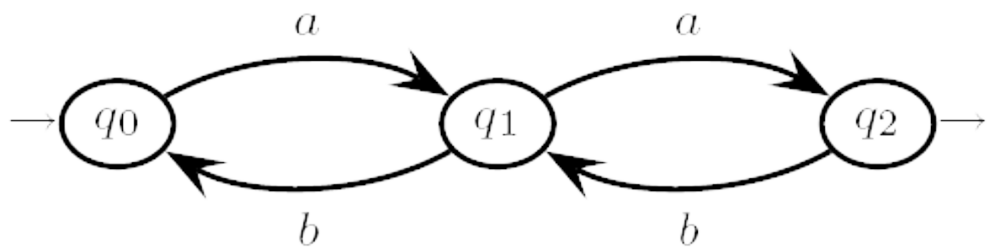
\includegraphics[width=0.5\linewidth]{images/compl.png}
    \end{figure}
    To find the complement automaton we have to add the error state $p$, obtaining the following automaton: 
    \begin{figure}[H]
        \centering
        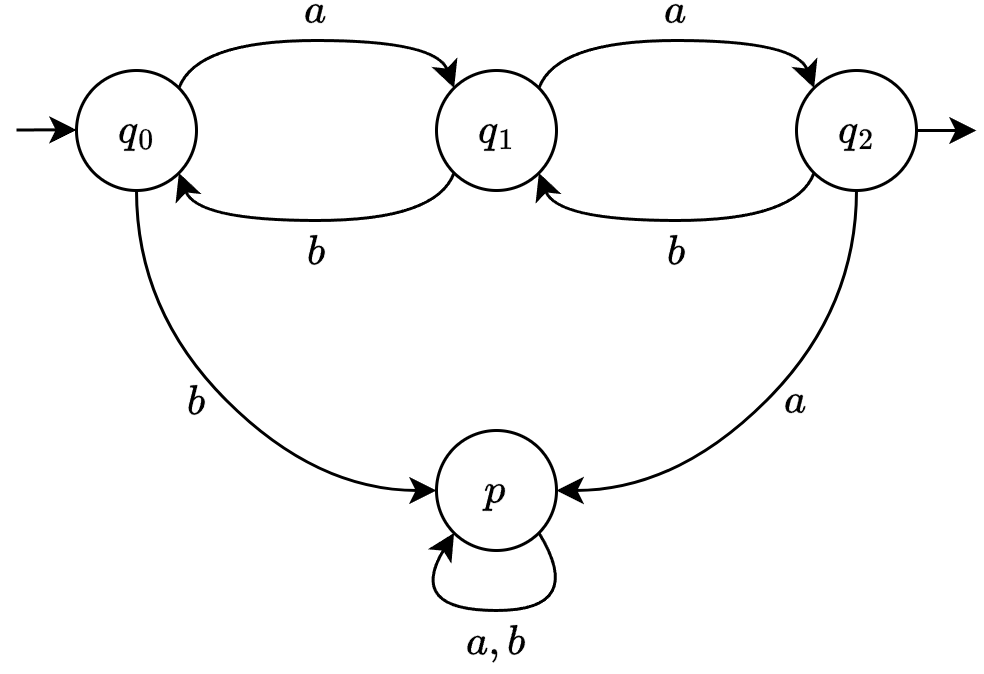
\includegraphics[width=0.35\linewidth]{images/compl1.png}
    \end{figure}
    Finally, we can swap final and non-final states: 
    \begin{figure}[H]
        \centering
        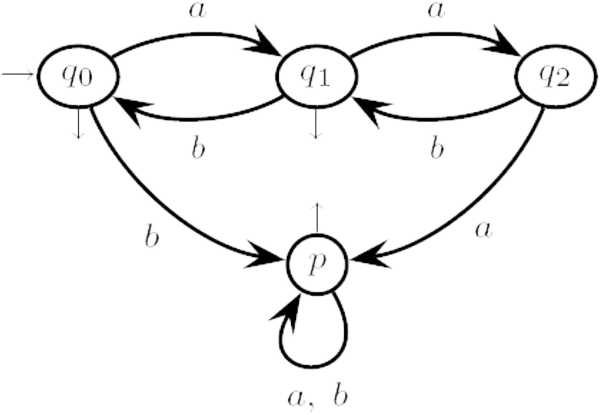
\includegraphics[width=0.35\linewidth]{images/compl2.png}
    \end{figure}
\end{example}
For the complement construction to work correctly, the original automaton must be deterministic, otherwise the original and complement languages may be not disjoint, which fact would be in violation of the complement definition. 
The complement automaton may contain useless states and may not be in the minimal form either; it should be reduced and minimized, if necessary. 

\subsection*{Cartesian product}
The product is a very common construction of formal languages, where a single automaton simulates the computation of two automata that work in parallel on the same input string. 
It is very useful to construct the intersection automaton. 
To obtain the intersection automaton we can resort to the De Morgan theorem: 
\begin{enumerate}
    \item Construct the deterministic recognizers of the two languages.
    \item Construct the respective complement automata. 
    \item Construct their union (Thompson). 
    \item Make deterministic the union automaton (Berry-Sethi). 
    \item Complement again and thus obtain the intersection automaton. 
\end{enumerate}

Since the intersection of the two languages is recognized directly by the Cartesian product of their automata, we can obtain the intersection automaton directly. 
Suppose both automata do not contain any spontaneous moves. 
The state set of the product machine is the Cartesian product of the state sets of the two automata. 
Each product state is a pair $\left\langle q^{'},q^{''} \right\rangle $, where the left (right) member is a state of the first (second) machine. 
The move is: 
\[\left\langle q^{'},q^{''} \right\rangle \overset{a}{\rightarrow} \left\langle r^{'},r^{''} \right\rangle \textnormal{ if and only if } q^{'} \overset{a}{\rightarrow} r^{'} \textnormal{ and } q^{''} \overset{a}{\rightarrow} r^{''}\]
The product machine has a move if and only if the projection of such a move onto the left (right) component is a move of the first (second) automaton. 
The initial and final state sets are the Cartesian products of the initial and final state sets of the two automata, respectively. 
\begin{example}
    Consider the languages $L^{'}=(a|b)^{*}ab(a|b)^{*}$ and $L^{''}=(a|b)^{*}ba(a|b)^{*}$. 
    The deterministic automaton for the language $L^{'}$ is as follows: 
    \begin{figure}[H]
        \centering
        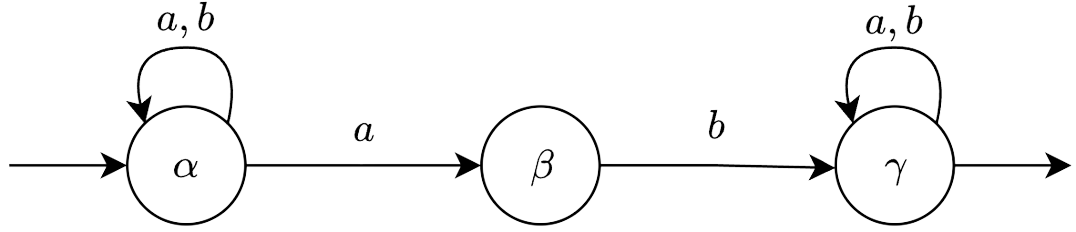
\includegraphics[width=0.5\linewidth]{images/int.png}
    \end{figure}
    And the deterministic automaton for the language $L^{''}$ is as follows: 
    \begin{figure}[H]
        \centering
        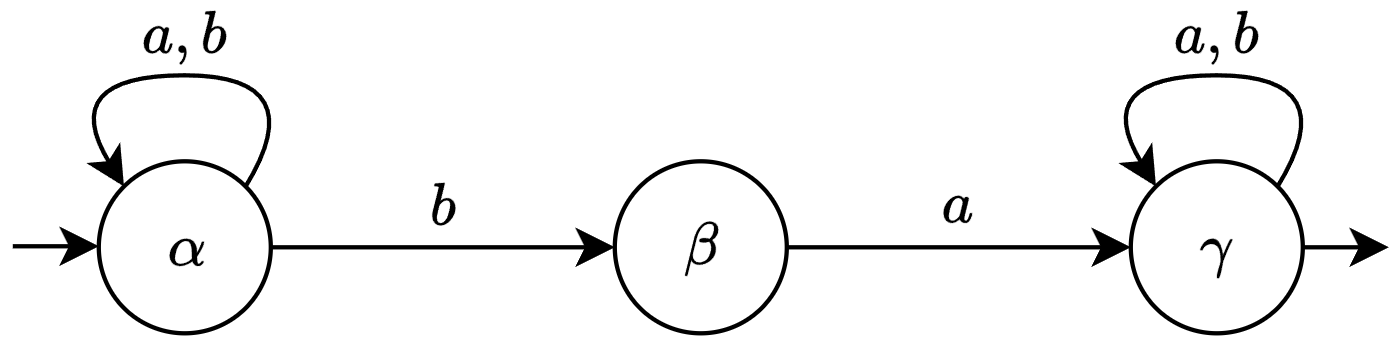
\includegraphics[width=0.5\linewidth]{images/int1.png}
    \end{figure}
    The intersection of the two is found with the following table: 
    \begin{figure}[H]
        \centering
        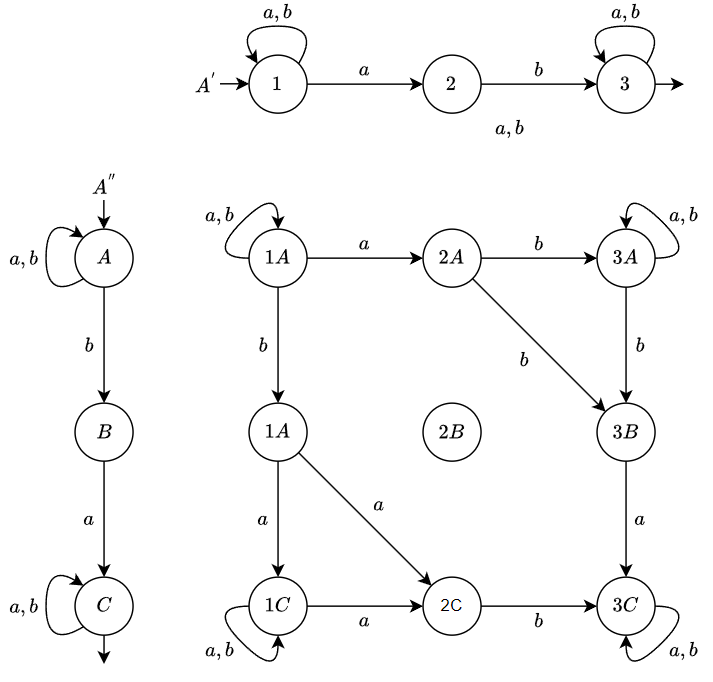
\includegraphics[width=0.75\linewidth]{images/int2.png}
    \end{figure}
\end{example}